\subsection{Testing}

This module is tested using a data loop-back test. Input data is transmitted through \textbf{uart\_tx\_line} and the transmitted signal is fed back into \textbf{uart\_rx\_line}. A testbench is used to do the loop-back testing. The signals within the testbench is denoted with \_tb suffice. Modelsim is used to simulated the module.

\subsubsection{8 Bit Mode}

\chapter{Documentations}


\section{Functional Block Diagram for Micro-controller}
The detail block diagram for the micro-controller designed in this research is as follows
\begin{figure}[!h]
	\centering
	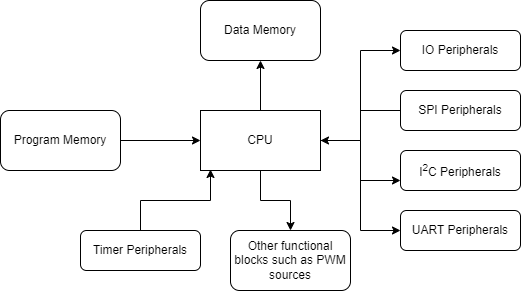
\includegraphics[scale=0.5]{/block_diagrams/functional_blocks}
	\caption{Functional Block Diagram for Micro-controller}
\end{figure}

\section{Functional Block Diagram for CPU}
The detail block diagram for the CPU designed in this research is as follows
\begin{figure}[!h]
	\centering
	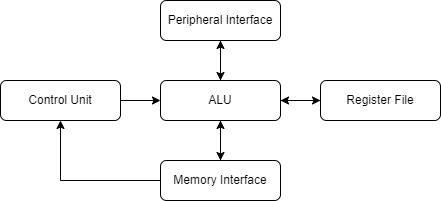
\includegraphics[scale=0.5]{/block_diagrams/functional_blocks_CPU}
	\caption{Functional Block Diagram for CPU}
\end{figure}
